\section{Efficiently Cleaning a Sample} \label{sampling}
%\reminder{Make sure that we do a good survey on ``sampling from a view'' and discuss them in the related work, e.g., [Frank et al., VLDB 86], [Nirkhiwale et al., VLDB 13]}
In this section, we describe how to find a relational expression $\mathcal{C}$ derived from the maintenance strategy $\mathcal{M}$ that
efficiently cleans a sample of a stale view $\widehat{S}$ and produces a sample of the up-to-date view $\widehat{S}'$.

\subsection{Challenges}
To illustrate the challenges in deriving $\mathcal{C}$, we present two naive solutions to this problem that will not work. 
First, the maintenance strategy $\mathcal{M}$ can be thought of as a data cleaning procedure to clean these errors, since applying the strategy to a stale view $S$ and the delta relations $\partial \mathcal{D}$ returns an up-to-date view $S'$ without data error.
We could trivially apply $\mathcal{M}$ to the entire stale view $S$ and update it to $S'$, and then sample.
While the result is correct according to our problem formulation, it does not save us on any computation for maintenance.
The intent is that restricting cleaning (maintenance) to a sample requires less computation; thus avoiding materialization of up-to-date rows outside of the sample.Alternatively, we could just apply $\mathcal{M}$ to the stale sample $\widehat{S}$ and a sample of the delta relations $\widehat{\partial \mathcal{D}}$. 
However, for general maintenance strategies, $\mathcal{M}$ does not commute with sampling. 

\subsection{Provenance}
\label{lin}
We explore the commutativity problem in more detail.
Consider the case of maintaining a view that is a group by aggregate:
\begin{lstlisting} [mathescape,basicstyle={\scriptsize}]
SELECT videoId, count(1) 
FROM Log
GROUP BY videoId
\end{lstlisting}
The resulting view has one row for every distinct videoId.
We want to materialize a sample of $S'$, that is a sample of videos with up-to-date counts.
If we randomly sample the delta relations $\widehat{\partial \mathcal{D}}$, we get a subset of records from LogIns.
The problem is that if we propagate the updates based on $\widehat{\partial \mathcal{D}}$ to $\widehat{S}$ it is not guaranteed that 
every count is completely up-to-date since we may not sample all the records for some groups.
This is because to achieve a sample of $S'$, we need to ensure that for each $s \in S'$ all contributing rows in subexpressions to $s$ are also sampled. 

This is a problem of row provenance \cite{DBLP:journals/vldb/CuiW03}.
Provenence, also termed lineage, has been an important tool in the analysis of materialized views \cite{DBLP:journals/vldb/CuiW03} and in approximate query processing \cite{DBLP:conf/sigmod/ZengGMZ14}.
\begin{definition}[Provenance]\label{prov}
Let $r$ be a row in relation $R$, let $R$ be derived from some other
relation $R = exp(U)$ where $exp(\cdot)$ be a relational
expression composed of the expressions defined in Section \ref{notation}.
The provenance of row $r$ with respect to $U$ is $p_U(r)$. 
This defined as the set of rows in $U$ such that for an update to any row $u \not\in p_U(r)$, it guarantees that $r$ is unchanged.
\end{definition}

\subsection{Primary Keys}
For the relational expressions defined in the previous sections, this provenance is well defined and can be tracked using primary key rules that are enforced on
each subexpression \cite{DBLP:journals/vldb/CuiW03}. 
So each row will have a designated primary key that will propagate to the next level of the relational tree.
Formally, we recursively define a set of primary keys for all nodes in the expression tree:
\begin{definition} [Primary Key Generation]
For every relational expression $R$, we define the primary key attribute(s) of every expression to be:
\begin{itemize}[noitemsep]
\item Base Case: All relations (leaves) must have an attribute $p$ which is designated as a primary key. That uniquely identifies rows.
\item $\sigma_{\phi}(R)$: Primary key of the result is the primary key of R 
\item $\Pi_{(a_1,...,a_k)}(R)$: Primary key of the result is the primary key of R. The primary key must always be included in the projection.
\item $\bowtie_{\phi (r1,r2)}(R_1,R_2)$: The primary key of the result is the tuple of the primary keys of $R_1$ and $R_2$. 
\item $\gamma_{f,A}(R)$: The primary key of the result is the group by key $A$ (which may be a set of attributes).
\item $R_1 \cup R_2$: Primary key of the result is the union of the primary keys of $R_1$ and $R_2$
\item $R_1 \cap R_2$: Primary key of the result is the intersection of the primary keys of $R_1$ and $R_2$
\item $R_1 - R_2$: Primary key of the result is the primary key of $R_1$
\end{itemize}
For every node at the expression tree, these keys are guaranteed to uniquely identify a row.
\end{definition}
These rules define a constructive definition that can always be applied for our defined relational expressions. 
We only have to ensure that any projection operation $\Pi$ includes the operand's primary key, and enforcing this condition
defines an equivalent materialized view.
As we will subsequently see, this primary key definition allows us to efficiently sample the relational expression.
For the relational expressions defined in the previous section, this method will always work.
However, in the future, if we expand the allowed set of relational expressions there are some limitations which we defer to future work.

\begin{example}
A variant of our running example view that does not have a primary key is:
\begin{lstlisting}[mathescape,basicstyle={\scriptsize}]
CREATE VIEW visitView
AS SELECT count(1) as visitCount
FROM Log, Video
WHERE Log.videoId = Video.videoId
GROUP BY videoId, ownerId, language, duration
\end{lstlisting}

To ensure that this view has a primary key for all subexpression,
we add the primary key to the projection:
\begin{lstlisting}[mathescape,basicstyle={\scriptsize}]
CREATE VIEW visitView
AS SELECT videoId, ownerId, language, duration,
count(1) as visitCount
FROM Log, Video
WHERE Log.videoId = Video.videoId
GROUP BY videoId, ownerId, language, duration
\end{lstlisting}
These two views are equivalent, as any query that can be answered with the previous view can be answered with 
the new view with the additional attributes.

Suppose there is a base relation, such as \tbl{Log}, that is missing a primary key (sessionId)\footnote{It does not make sense for Video to be missing a primary key in our running example due to the foreign key relationship}.
We can add this attribute by generating an increasing sequence of integers for each record in \tbl{Log}.
Then, we can apply the rules above to propagate this key up the expression tree.
\end{example}

\subsection{Hashing Operator}
\label{push}
These primary keys define the provenance of a row $r$, which allows us to easily determine the set of rows in subexpressions that contribute
to $r$:
\begin{proposition}[Primary Key Provenance]\label{provalg}
Let $R$ and $U$ be relations as defined in Definition \ref{prov}. 
Let $A_R$ be the primary key set of $R$ and $A_U$ be the primary key 
set of $U$.
Define $r(A_R)$ as the primary key sets values for the row $r$.
$p_U(r)$ is defined as follows: (1) if $A_R \subseteq A_U$ then 
$\{u \in U: u(A_R) = r(A_R)\}$, (2) if $A_R \not \subseteq A_U$ then
return $U$.
\end{proposition}
We now explore how we can design a sampling technique to guarantee that all of the rows in Proposition \ref{provalg} are sampled if $r$ is sampled.
If we have a deterministic way of mapping a primary key defined in the previous subsection to Boolean true or false, we can ensure that all contributing rows are also sampled. 
To achieve this we use a hashing procedure.
Let us denote the hashing operator $\eta_{a, m}(R)$. 
For all tuples in R, this operator applies a hash function whose range is $[0,1]$ to primary key $a$ (which may be a set) and selects those records with hash value less than or equal to $m$.
If the hash function is sufficiently uniform, then the condition $h(a) \le m$ is true for close to a fraction $m$ of the rows. 
%This definition is without loss of generality for uniform hash function, as if we have a hash function whose range is the set of integers (as implemented in MySQL or Apache Hive) we can take the absolute value and divide by the maximum integer mapping this range back $[0,1]$. 

We push down the hashing operator through the query tree.
The further that we can push $\eta$ down the expression tree, the more operators can benefit from the sampling.
However, it is important to note that for some of the expressions, notably joins, the push down rules are more complex. 
It turns out in general we cannot push down even a deterministic sample through those expressions.
We formalize the push down rules below:
\begin{definition}[Hash Pushdown]
Let $a$ be a primary key of a materialized view. The following rules can be applied to push $\eta_{a, m}(R)$ down the expression tree of the maintenance strategy. 
\begin{itemize}[noitemsep]
\item $\sigma_{\phi}(R)$: Push $\eta$ through the expression.  
\item $\Pi_{(a_1,...,a_k)}(R)$: Push $\eta $ through if $a$ is in the projection.
\item $\bowtie_{\phi (r1,r2)}(R_1,R_2)$: Blocks $\eta $ in general. There are special cases below where push down is possible.
\item $\gamma_{f,A}(R)$: Push $\eta $ through if $a$ is in the group by clause $A$.
\item $R_1 \cup R_2$: Push $\eta $ through to both $R_1$ and $R_2$
\item $R_1 \cap R_2$: Push $\eta $ through to both $R_1$ and $R_2$
\item $R_1 - R_2$: Push $\eta $ through to both $R_1$ and $R_2$
\end{itemize}
\end{definition}
In special cases, we can push the hashing operator down through joins. 
Given the hash function $\eta_{a, m}(R)$:
\vspace{.25em}

{\noindent \textbf{Equality Join:}} If the join is an equality join and $a$ is one of the attributes in the equality join condition $R_1.a = R_2.b$, then $\eta$ can be pushed down to both $R_1$ and $R_2$. On $R_1$ the pushed down operator is $\eta_{a, m}(R_1)$ and on $R_2$ the operator is $\eta_{b, m}(R_2)$. This case often happens near the top of maintenance strategy expression tree where there is a equality outer join on the primary key of the stale view and a ``delta view''.

\vspace{.25em}

{\noindent \textbf{Foreign Key Join:}} If we have a join with two foreign-key relations $R_1$ (fact table with foreign key $a$) and $R_2$ (dimension table with primary key $b \subseteq a$) and we are sampling the key $a$, then we can push the sampling down to $R_1$. This is because we are guaranteed that for every $r_1\in R_1$ there is only one $r_2 \in R_2$. This case happens in our running example. If we sample the view on the primary key (\texttt{videoId}, \texttt{ownerId}, \texttt{language}, \texttt{duration}), since each video has only one owner, language and duration, we can push down the sampling of \texttt{videoId} to the \tbl{Log} relation and the \tbl{LogIns} table.

%A special case of the equality join rule is if we have a join with two foreign-key relations $R_1$ (fact table) and $R_2$ (dimension table). If we are sampling the foreign key (the primary key of the dimension table), then we can push down $\eta$ to both relations as in the equality join case. 

%\vspace{.25em}

%{\noindent \textbf{(Semi/Anti)-Join:}} Similarly, if we are hashing the primary key of a semi-join, we can always push $\eta$ down $R_1$. For anti-joins we can push $\eta$ down because we can rewrite the node as $R_1 - (R_1 \ltimes R_2) $ and apply the pushdown rules for set difference and Semi-Joins.

\vspace{0.25em}

The result of this hash operator pushdown on $\mathcal{M}$ is the cleaning expression $\mathcal{C}$. 
When applied to a stale sample of a view $\widehat{S}$, the database $\mathcal{D}$, and the delta relations $\partial \mathcal{D}$, it produces an up-to-date sample with sampling ratio $m$:
\[
\widehat{S}' = \mathcal{C}(\widehat{S},\mathcal{D},\partial \mathcal{D})
\]
Thus, it addresses Problem 1 from the previous section.

\subsection{Corresponding Samples}
We started with a uniform random sample $\widehat{S}$ of the stale view $S$.
The hash push down allows us to efficiently materialize the sample $\widehat{S}'$.
$\widehat{S}'$ is a uniform random sample of the up-to-date view S.
While both of these samples are uniform random samples of their respective relations, 
the two samples are correlated since $\widehat{S}'$ is generated by cleaning $\widehat{S}$.
In particular, our hashing technique ensures that the primary keys in $\widehat{S}'$ depend on the primary keys in $\widehat{S}$.
Statistically, this positively correlates the query result $q(\widehat{S}')$ and $q(\widehat{S})$. 
We will see how this property can be leveraged to improve query estimation accuracy (Section \ref{re}). 

We call this property correspondence:
\begin{property}[Correspondence]
Suppose $\widehat{S'}$ and $\widehat{S}$ are uniform samples of $S'$ and $S$, respectively.  Let $u$ denote the primary key. We say $\widehat{S'}$ and $\widehat{S}$ correspond if and only if:
\vspace{-.25em}
\begin{itemize}[noitemsep]
\item Uniformity: $\widehat{S'}$ and $\widehat{S}$ are uniform random samples of $S'$ and $S$ respectively with a sampling ratio of $m$
\item Removal of Superfluous Rows: $D = \{\forall u \in \widehat{S} \wedge u \not\in S'\}$, $D \cap \widehat{S'} = \emptyset$ 
\item Sampling of Missing Rows: $I = \{\forall u \not\in S : u \not \in S\}$, \[\mathbb{E}(\mid I \cup \widehat{S'} \mid) = m\mid I \mid \]
\item Key Preservation: For all $u\in \widehat{S}$ and not in $D$ or $I$, $u\in \widehat{S}'$.
\end{itemize}
\vspace{-.25em}
\label{correspondence}
\end{property}

\subsection{Example}
We illustrate our proposed approach on our example view \texttt{visitView} (Figure \ref{exexpr2}). 
The primary key for the view is the tuple (\texttt{videoId}, \texttt{ownerId}, \texttt{language}, \texttt{duration}) making that the primary key of the MV.
We can apply our hash operator to this key, and use the pushdown rules described in Section \ref{push} to efficiently sample the maintenance strategy. 
We start by applying the hashing operator to this key.
The next operator we see in the expression tree is a projection that increments the \texttt{visitCount} in the view, and this allows
for push down since primary key is in the projection.
The second expression is a hash of the equality join key which merges the aggregate from the ``delta view'' to the old view allowing us to push down on both branches of the tree using our special case for equality joins.
On the left side, we reach the stale view so we stop.
On the right side, we reach the aggregate query (count) and since the primary key is in group by clause, we can push down the sampling.
Then, we reach another point where we hash the equality join key allowing us to push down the sampling to the relations \tbl{LogIns} and \tbl{Video}.
In terms of increased efficiency, since both the aggregation and joins are ``above'' the sampling operator, they require less computation and less memory.

\begin{figure}[t] \vspace{-2em}
\centering
 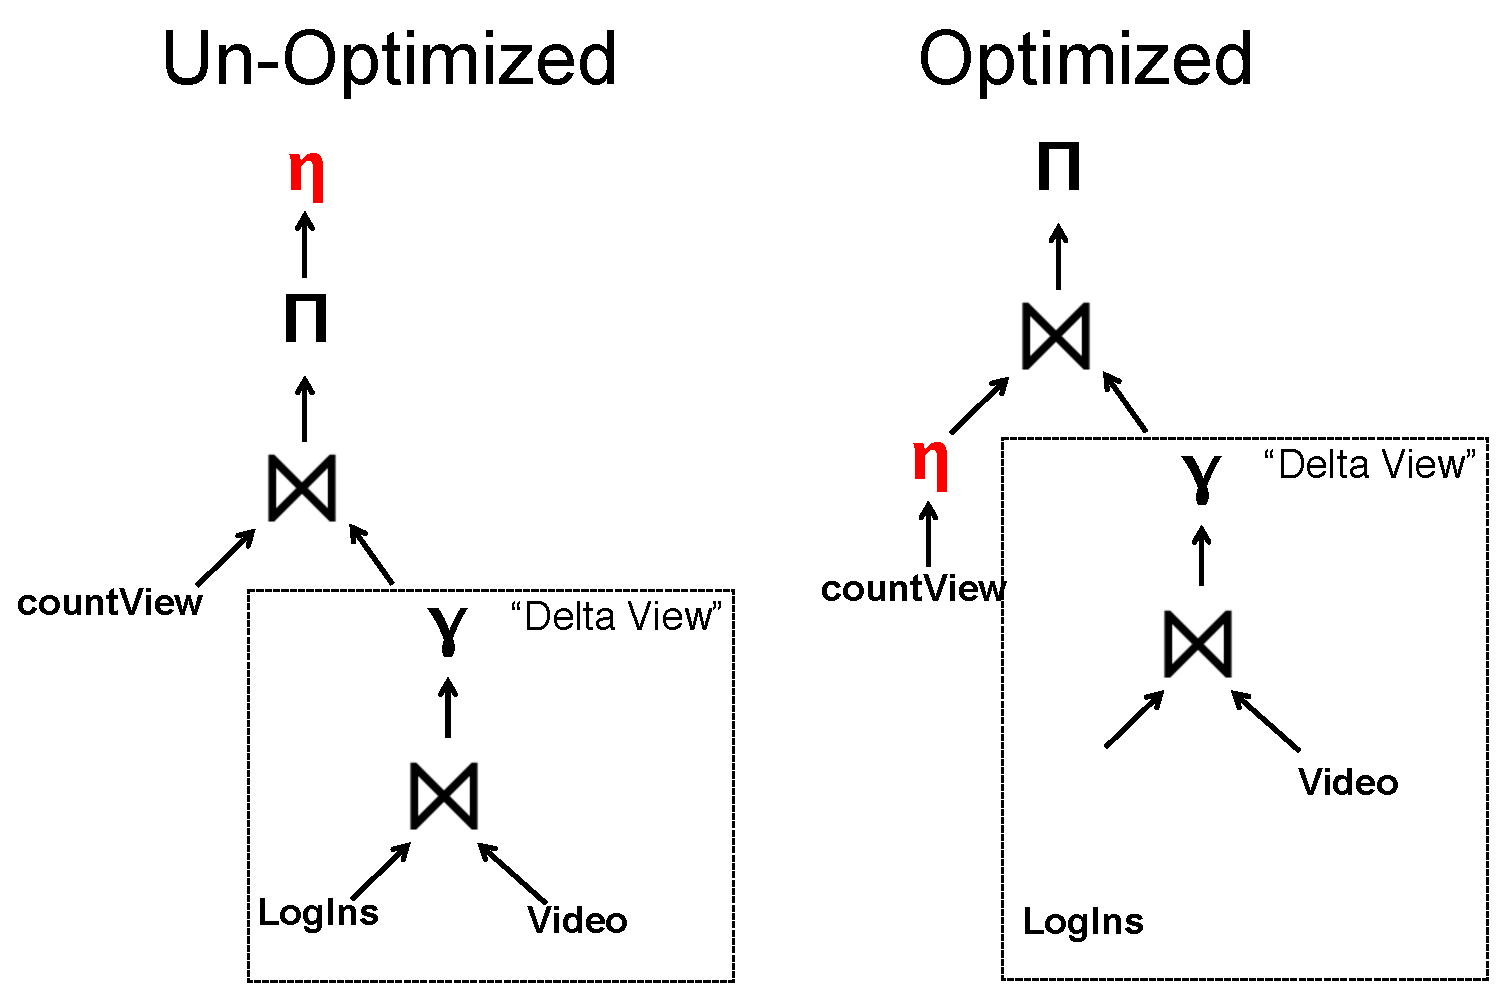
\includegraphics[scale=0.24]{figs/example_expression_tree_2.pdf} \vspace{-.5em}
 \caption{Applying the rules described in Section \ref{push}, we illustrate how to optimize the sampling of our example maintenance strategy. \label{exexpr2}}\vspace{-1.75em}
\end{figure}




